\documentclass{beamer}
\usepackage{amsmath,listings,pifont,multirow}
%\usepackage{pgf,pgfarrows,pgfnodes,tikz}

\newcommand{\chk}{\ding{51}}
\newcommand{\ex}{\ding{55}}

\setbeamercovered{transparent}
\usetheme{Luebeck}

\mode<presentation>
\setbeamertemplate{navigation symbols}{}

\lstset{language=ML}

\title[Higher-Order Modules, Sep. Comp., and Signatures]{True Higher-Order Modules, Separate Compilation, and Signature Calculi}
\author{George Kuan}
\institute{University of Chicago}
%\date{Candidacy Exam\\January 15, 2009}
\date{PL Seminar\\March 6, 2009}

\begin{document}

\begin{frame}
  \titlepage
\end{frame}
% Thank you for coming

% \begin{frame}
% \frametitle{What's Wrong With Modern Module System Design}
% \begin{enumerate}
% 	\itemsep=1.5cm
% \item ``True'' higher-order functors
% \item ``True'' separate compilation
% \item Signature language
% \end{enumerate}
% \end{frame}
% The main issues my dissertation will address is the design and semantics of true higher-order functors
% Closely related to higher-order functors is the problem of separate compilation
% Finally, both of the above rely on the richness of the signature language, which I also seek to improve in a general sense 

\section{Higher-Order Functors}

\begin{frame}[fragile]
\frametitle{Why Higher-Order Functors?}
\begin{lstlisting}
functor F() = struct ... end
functor G() = 
struct
  structure M = F()
end
	
functor G'(functor F() : sig end) =
struct
  structure M = F()
end
\end{lstlisting}	
Commentary on Standard ML: Separate compilation and abstraction over functors
\end{frame}
% functors are not closed with respect to modules identifiers 

\begin{frame}[fragile]
\frametitle{Why Higher-Order Functors?}
Indefinite references to functors 

\begin{block}{In action: simple and succinct extensions of functors (Biswas 95)}
%Higher-order functors promote . 
\begin{lstlisting}
functor RedBlackSetFn(K:ORD_KEY) ...
functor ExtSetFn
  (functor SetFn(Ord:ORD_KEY): ORD_SET) 
  (K:ORD_KEY) =
struct
  structure M = SetFn(K)
  open M
  (* Extensions to SetFn *)
  type ...
  val ...
end 	
\end{lstlisting}
\end{block}	 
\end{frame}
% In module systems, functors permit us to reference indefinite structures, to support better code factoring and reuse. It is natural to take this principle up a level. Higher-order functors enable programmers to make indefinite reference to functors. 
% One specific and narrow example is given here. Basis functors can be extended without touching the Basis itself by a higher-order functor that takes a Basis functor as an argument.

\begin{frame}[fragile]
\frametitle{Full Transparency in Higher-Order Functors}

\begin{lstlisting}
functor Apply(functor F(X:sig type t end) 
                      : sig type t end) 
             (M : sig type t end)	
  = F(M)
\end{lstlisting}
% What happens if formal functor is transparent but argument is opaque?
% SML/NJ seems to permit it, giving the opaque structure as the result.
% Formal functors can't be opaque anyway. Why is this the case?

\begin{lstlisting}
functor Id(X : sig type t end) 
  = struct type t = X.t end

structure M = Apply(functor F=Id)
                   (struct type t = int end)
\end{lstlisting}
\begin{block}{}
\only<1>{???}
\only<2->{\lstinline{structure M : sig type t end}} \only<3>{\alert{Too conservative!}}
\end{block}
\end{frame}
% One of the main challenges in higher-order functors is the problem of full transparency. I will illustrate this property with a few examples
% The apply functor is the canonical example for higher-order functors
% Given an identity functor as an argument, what should the Apply functor return? If we just naively follow the given formal functor signature, we can only give a very conservative opaque signature. 


\begin{frame}[fragile]
\frametitle{Full Transparency in Higher-Order Functors}
\begin{lstlisting}
functor Apply(functor F(X:sig type t end) 
                      : sig type t=X.t end) 
             (M : sig type t end)	
  = F(M)
\end{lstlisting}

\begin{lstlisting}
functor Id(X : sig type t end) 
  = struct type t = X.t end

structure M = Apply(functor F=Id)
                   (struct type t = int end)
\end{lstlisting}
\begin{block}{}
\only<1>{???}
\only<2->{\lstinline{structure M : sig type t = int end}} \only<3>{\alert{Too restrictive!}}	
\end{block}
\end{frame}
% We can strengthen the formal functor signature by adding a definitional spec that mirrors the type propagation that is going on in the Identity functor. Now, the int type gets propagated through as per the semantics of the Identity functor. 

\begin{frame}[fragile]
\frametitle{Full Transparency in Higher-Order Functors}
\begin{lstlisting}
functor Apply(functor F(X:sig type t end) 
                      : sig type t=X.t end) 
             (M : sig type t end)	
  = F(M)
\end{lstlisting} 

\begin{lstlisting}
functor K(X : sig type t end) 
  = struct type t = int end	

structure M = Apply(functor F=K)
                   (struct type t = int end)
\end{lstlisting}
\begin{block}{}
\only<1>{???}
\only<2>{Signatures of formal functor F and K don't match}	
\end{block}
\end{frame}
% Unfortunately, we strengthened the formal functor signature too much. The Apply functor was supposed to be a general Apply functor, but we strengthened the formal functor signature such that it only matches the Identity functor. If I tried to apply the Apply functor to any other argument functor such as the Constant functor, the program would fail to typecheck. 


\begin{frame}
\frametitle{Full Transparency in Higher-Order Functors}
\begin{definition}[Type Action]
	The way in which a functor computes its output types from its parameter types including generativity and actions of formal functor components
\end{definition}
\begin{definition}[Full Transparency]
	The propagation of all \alert{type actions} in a functor through higher-order functor applications. 	
\end{definition}
\begin{definition}[True Higher-Order Functors]
True higher-order functors respect the \alert{full transparency} property. 
\end{definition}
\end{frame}
% In summary, a functor can do different things to compute output types from parameter types. This is not limited to pretty nontrivial operations such as generativity and actions. We call this computation the type action of the functor. 
% Full transparency is the propagation of all the type actions. The underlying principle here is that functor application must respect all the type actions in that functor. 


\begin{frame}[fragile]
\frametitle{Applicative Functors (Leroy 95)}
Type equivalence = path equivalence\\
Notion of paths extended to application of functor to another path \lstinline{F(M).t}\\
Need theory of equality of paths\\ %% Such as???
\begin{lstlisting}
Apply : functor(functor F(X:sig type t end) 
                        : sig type t end) 
               (structure M : sig type t end) 
          : sig type t = F(M).t end
\end{lstlisting}	
\end{frame}
% One popular solution to this problem is Leroy's applicative functor semantics. Based on the manifest types paper's idea that path equivalence can be considered a kind of type equivalence. However, in the case of higher-order functors type propagation cannot be expressed in terms of a definitional spec on a simple path as we've seen in the earlier example. Leroy's main idea is to enrich his notion of paths with rooted functor applications, e.g. F(M).t. Under this semantics, the types from the result of two functor applications are equivalent if they are the same functor to the same argument. There is a bit of a design space in terms of what consitutes the ``same'' argument module, but the simplest solution is to fall back on path equivalence. Using this semantics, we can give the Apply functor the following signature that expresses the dependency of the result type t on the formal functor type action. 

\begin{frame}[fragile]
\frametitle{Shortcomings of Applicative Functors}
\begin{block}{Lacks generative semantics}
\begin{lstlisting}
functor SymbolTable() = 
  struct type symbol = int ... end 
  :> sig type symbol ... end
\end{lstlisting}
\end{block}
\end{frame}
% Although applicative functors are fairly widely adopted, they are not without their own problems. One widely recognized issue is that the semantics drops support for the more traditional generative semantics of classic ML functors. Generative semantics are useful as is the case with this example. The symboltable functor produces a hashtable index by integer symbols. We don't want this implementation detail to leak out, but under applicative semantics, the symbols from one symboltable can be used to indexed the other because they were instantiated with identical arguments, i.e., the empty argument. Generative functors would appropriately generate fresh types for each instantiation and thereby maintain this desirable abstraction. 

\begin{frame}[fragile]
\frametitle{Shortcomings of Applicative Functors}
\begin{block}{Functor applications in paths must be A-normalized}
\begin{lstlisting}
signature T = sig type t end

functor:
  functor ApplyToInt(functor G(X:T):T) = 
    G(struct type t = int end)

signature: 
  functor ApplyToInt(functor G: (X:T):T) : T

structure R = ApplyToInt(functor G = Id)
\end{lstlisting}
% structure FR : 
%   sig
%     functor H(M:T) : sig type t = Id(M).t end
%     structure R : sig type t = F(Id).R.t end
%   end

\lstinline{val x : R.t = 42} \alert{int mismatch R.t = ApplyToInt(Id).t}
\end{block}	
\end{frame}
% The other shortcoming is not as widely cited is the fundamental problem of typechecking using only syntactic paths. Such an approach to typechecking necessitates A-normalization of all functor applications. Such as transformation would make error messages more difficult to decipher and clutter up code. As we show in this example, an un-A normalized HO functor application leads to problems. Without a path for the argument to the functor G, we can't ascribe a signature richer than the most conservative sig type t end. Furthermore, we don't have any details about G but have to give a signature for F right then. This disrupts the type propagation in the program. By the time we see G is Id, it is too late. F already received the more conservative signature. 

\begin{frame}
\frametitle{Design Space}
\begin{enumerate}
	\itemsep=1cm
	\item Applicative functors (OCaml)
	\item Include both applicative and generative functors (Moscow ML, DCH)
	\item \ldots
\end{enumerate}	
\end{frame}

\begin{frame}[fragile]
\frametitle{True Higher-Order Functors}
\begin{description}
	\itemsep=1cm
\item[Alternative:] Fully transparent generative higher-order functors
\item[Examples:] Re-elaboration semantics (MacQueen and Tofte 94) and internal language semantic representation static lambda calculus (implicitly in SML/NJ) % expressive of type actions modulo generativity
\end{description}
\begin{block}{Claim}
\begin{enumerate}
	\itemsep=0.7cm
	\item True HO functor semantics is exactly what we want
	\item Applicative functors are an ``in-between'' approximation
\end{enumerate} 
\end{block}
\end{frame}
% The alternative to applicative functors is to return to generative functors and extend their semantics to account for full transparency. The desired solution is fully transparent generative HO functors. This semantics is embodied in the MacQueen and Tofte 94 paper that used re-elaboration, i.e., re-elaborate the functor body at the site of functor application. This requires the functor body to be available at the point of application. The compiler has refined this approach significantly by actually compiling the functor body into a static lambda calculus that encodes what is necessary to reproduce the type action of that functor so we don't need the whole functor body to typecheck applications. The static lambda calculus plus generativity expresses the type actions of functors. Our tenative claim is that the semantics of these true HO functors is exactly what we want. It does full type propagation (i.e., full transparency) while maintaining the desirable generative semantics of functors to maintain abstractions in certain cases. Applicative functors, on the other hand, supports full transparency in many cases but breaks down wrt generativity and the remaining cases.

%% In first-order case, we can compensate for loss of type information by presence of operators, can be approximated and reconstructed using simple definitions
%% In higher-order case, the loss of type actions is too much to compensate for

% Question: Why not use internal semantic representation for surface signature language?

\begin{frame}
\frametitle{True Higher-Order Functors}
\begin{block}{Why are they much more difficult than the first-order case?}
\begin{itemize}
	\item First-order: hide abstract types - access by interface of functions
	\item Higher-order: hide type action - ??? 
\end{itemize}	
\end{block}	
\end{frame}

\section{Separate Compilation}
\begin{frame}
\frametitle{Separate Compilation}
\begin{block}{Key Problem}
	True higher-order functors do not seem to be compatible with true separate compilation. The signature language cannot describe type action propagation adequately in functor signatures.
\end{block}
\end{frame}
% The main disadvantage to true HO functors is that re-elaboration semantics seems to conflict with true separate compilation in the style of Modula-2. In Modula-2, there is a clear distinction made between self-contained interfaces and implementation. Under re-elaboration semantics, the interface language, signatures, are not sufficient by themselves for separate typechecking. 

\begin{frame}
\frametitle{Definition of True Separate Compilation}
\begin{block}{Cardelli 97}
True separate compilation is the ability to separately typecheck program fragments in the presence of a local environment (a set of explicit interfaces) such that the fragments can be safely linked together.
\end{block}	
\end{frame}
% Cardelli gave one of the few formal accounts of true separate compilation. The key idea is that the compiler can separate compile (of which typechecking is the most important part) program fragments, modules, with only the aid of a set external interfaces. The resulting types can then be checked for consistency in order to link the modules together. 

\begin{frame}
\frametitle{True Separate Compilation}
\begin{block}{Conjecture}
True HO functors and true separate compilation are mutually exclusive
\end{block}
\vspace{1cm}
Reasoning: Intuitively, necessary signature and type language too complex...Should be fairly straightforward
% Techniques: strong sums model predicts full transparency
% Typechecking for a language with both features is undecidable?
% (*) By construction
% Decidability of full propagating type system unclear
% 
\end{frame}
% The conjecture I will make for my dissertation is that true HO functors and true separate compilation are in fundamental conflict. They are mutually exclusive because of the intuition that the signature language cannot be made rich enough to encode all the possible type actions of functors. 

\section{Signature Calculi}

\begin{frame}[fragile]
\frametitle{Signature Calculi}

The ML signature language is a simple interface language with support for signature extension (syntactic \lstinline{include}), hierarchical nesting, where type clauses, and type sharing constraints.\\[1cm]

But as Ramsey {\it et al.} 05 and Garcia {\it et al.} 05 noted, richer extensions would be useful. 
\end{frame}
% Since I will be studying enriching the signature anyway, I will revisit the ML signature language in order to enrich it in a more general sense. The signature language has a few facilities for controlling and constraining structures, but as others have noted, it should be enriched to support more flexible signature composition. As it stands, the signature language in the Def'n is limited. One must often copy and paste, maintaining separate signatures that otherwise share content. What we need is language support for signature extension.

\begin{frame}[fragile]
\frametitle{SML/NJ Implementation of Signature Extension}
\begin{lstlisting}
signature S2 = sig
  include S0
  include S1 
end	
\end{lstlisting}
\begin{tabular}{ll|l|l|l|l|}
%\hline
 \multicolumn{2}{c}{} & \multicolumn{4}{c}{S0}\\
%\hline
  \multicolumn{2}{c|}{}    & type & eqtype & datatype & deftype \\
\hline 
\multirow{4}{*}{S1} & type & \chk & eqtype & \ex & \ex\\
 % \hline
 & eqtype & type & \chk & \ex & \ex\\
 %\hline
 & datatype & \chk & datatype & \ex & \ex\\
 %\hline
 & deftype & \ex & \ex & \ex & \ex\\
\hline
\end{tabular} \\
SML/NJ signature elaboration compatible signature merging: \chk~can be merged, \ex~cannot be merged, otherwise indicates specs merge-able but indicated spec takes precedence
	
\end{frame}
% SML/NJ's signature elaboration attempts to do a little more than what is required by the Def'n. It does not reject offhand when two included signatures have overlapping components. Instead, elaborator attempts to merge these components when they are compatible. The current merging algorithm is ad hoc and inconsistent in places. For example, merging eqtype and type results in a different spec depending on the order of inclusion. Deftypes can never be merged with types. Eqtypes and datatypes can be sometimes unsoundly merged while they are considered incompatible in the other direction. 

% Questions: What are some implications of merging deftype and type? 

\begin{frame}[fragile]
\frametitle{Ramsey {\it et al.} Signature Extension}

\begin{columns}
	\begin{column}{3cm}
\begin{lstlisting}[frame=none]
signature S0 =
sig
  type t
  type u 
  val x : t list
end
\end{lstlisting}
\end{column}
\begin{column}{3cm}
%\hspace{0.1cm}
\begin{lstlisting}[frame=none]
signature S1 = 
sig
  type t
  type u 
  val x : u list
end	
\end{lstlisting}
\end{column}
\end{columns}

\begin{lstlisting}[frame=none]
S0 andalso S1 =	
sig
  type t 
  type u = t
  val x : t list
end	
\end{lstlisting}	
\end{frame}
% Ramsey describes a semantics for compatible signature merging by an explicit andalso construct. In effort to find the least upper bound for the entirety of signatures, Ramsey's semantics is too aggressive, inferring definitional specifications where none existed before. This example merge should be rejected because the value specs cannot be reconciled short a draconian measure. 

\begin{frame}[fragile]
\frametitle{Signature Calculi (1)}	
\begin{block}{Merge}
\begin{lstlisting}
signature SIG0 = sig eqtype t end
signature SIG1 = sig type t = int end
signature SIG = 
sig 
  include SIG0
  include SIG1
end
\end{lstlisting}
\end{block}
\end{frame}

\begin{frame}[fragile]
\frametitle{Signature Calculi (2)}
\begin{block}{Access inferred signatures}
\begin{lstlisting}
structure M = 
struct 
  type t = int
end
signature S = sign(M)	
\end{lstlisting}	
\end{block}
\end{frame}
% In my dissertation I would like to design a sensible signature calculus that incorporates compatible signature merging and other features such as extensions using extracted or inferred signatures. In this example, sign(M) reduces to the inferred signature for M. Using this, a programming can build signatures out of the signatures implied by existing definite modules. 

% Question: Does access to inferred signature conflict with the phase distinction? 
% What are some practical uses for this inferred signature stuff?

\begin{frame}[fragile]
\frametitle{Signature Calculi (3)}
\begin{block}{Signature components in modules}
\begin{lstlisting}
structure Control = 
struct 
  signature PRINT = sig ... end 
  structure Print : PRINT = struct ... end 
  ... 
end
\end{lstlisting}
Structures should permit signature components for signatures that represent type classes. 
\end{block}
\end{frame}
% Another feature that might be interesting is permitting signature components in modules. In the compiler, when we have hierarchically nested modules such as Control, all the signature are still on the toplevel. Using module hierarchies to constrain signature scopes, we can enable more structured. 

% Question: Do signature components lead to any avoidance problems? 

\begin{frame}[fragile]
\frametitle{Signature Calculi (4)}
\begin{block}{Parameterized signatures}
\begin{lstlisting}
signature SIG0(M:sig type t end) 
  = sig type t = M.t end
\end{lstlisting}
\end{block}
For representing type classes: 
\begin{lstlisting}
signature Eq(type a) = sig
  val == : a -> a -> bool
end	
\end{lstlisting}
%signature SIG1(X) = sig structure M : X end	
% Interesting Question: How does this impact phase distinction?
\end{frame}
% One more feature novel to ML would be signatures parameterized on modules and perhaps other signatures. In the former case, the semantics seem straightforward. This provides another way to produce signature families perhaps more general than what is currently afford by the where type mechanism. Parameterizing signatures on signatures is significantly murkier. I will have to investigate how to constrain signatures (a kind of bounded subtyping polymorphism perhaps) such that the elaborator can get something useful out of the signature parameter. 

% \section{Research Plan}
% \begin{frame}
% \frametitle{Proposed Research Plan}
% \begin{enumerate}
% \item<1-> Formalization based on module elaboration in SML/NJ
% \only<1>{using elaboration semantics approach}
% \item<2-> Clarification of the semantics of true HO functors
% \item<3-> Classic type soundness for true HO functor semantics
% \item<4-> Prototype implementation (including possibly improved algorithms for elaboration)
% \item<5-> Formalization of mutual exclusion theorem (or a semantics that admits both separate compilation and true HO functors)
% \item<6-> Extensions for signature calculus and type soundness for module language with extended signature calculus
% %\item<7-> Connections to related ideas 
% \end{enumerate}	
% \end{frame}
% I intend to continue to develop my formalization of the module elaborator in SML/NJ. The goal of this research is to have not only a complete theoretical model but also a convenient surface module language. Although the semantics of true HO modules is implicit in the compiler, I seek to clarify the semantics, to clean up and simplify it where appropriate. I would also like to produce a classic type soundness proof for the resultant semantics. This is slightly different from the bulk of prior research which produced soundness proofs for the typechecking algorithm wrt to a given declarative type system. This simplified semantics should also be amenable to a prototype implementation that will serve as a platform for testing improved and simplified elaboration algorithms. Another key result would be a precise statement of the relationship between true separate compilation and true HO functors or a semantics that admits both. I will explore the enriching the signature language and its corresponding module system soundness. Finally, I will study the connections to the related concepts. 

% Question: Classic Type Soundness with elaboration semantics and semantic objects?
\section{Conclusion}
\begin{frame}
\frametitle{Related Work}
\begin{center}
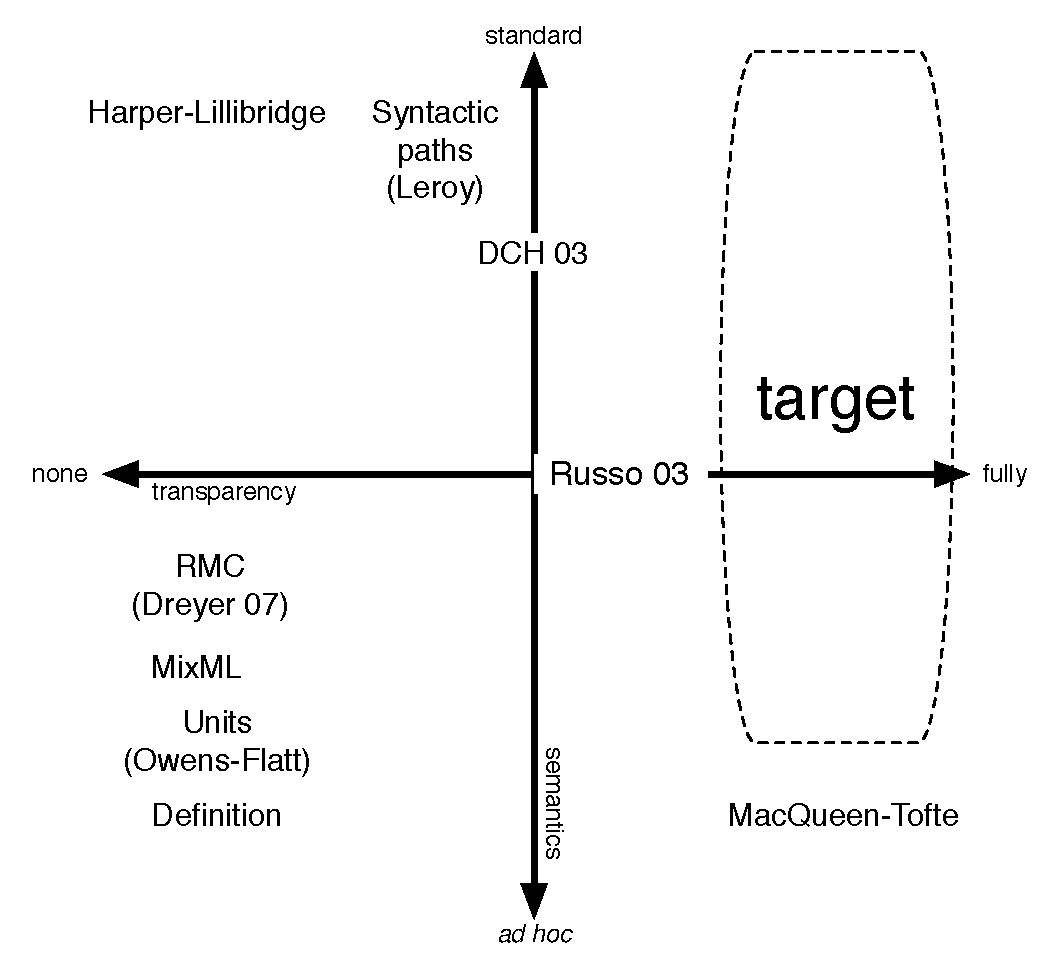
\includegraphics[scale=0.4]{../../../design/figs/modsys-spectrum.pdf}
\end{center}
\end{frame}
% There are a wide variety of module systems developed in the past few decades. In this figure, I will classify them based on whether they support full transparency with the various gradations standing in for the different combinations of applicative and generative functors. The vertical axis classifies the systems based on how close to some standard type theory they are. Most of the work has been in non-propagating and ad hoc semantics. Some of the early work attempted using fairly standard type theories to model non-propagating modules. The area on the upper right is fairly devoid of any development. I seek to explore this area. 

\begin{frame}
\frametitle{Conclusion}	
\begin{enumerate}
	\itemsep=0.5cm
	\item Static and dynamic semantics for true HO modules based on SML/NJ and recent module system designs
	%\item Precise account of true HO functors versus separate compilation
	\item Signature calculi with compatible merges and other signature manipulation elements
	%\item Exploration of how related constructs such as type classes, FCP type inference, and mixins fit together 
	\item Towards a Successor ML
\end{enumerate}
\end{frame}
% To conclude, the dissertation I am proposing will develop static and dynamic semantics for true HO functors based on SML/NJ's implementation. It will provide formal accounts of the tension between true HO functors and SC. Finally, I will enrich the signature calculi and explore various related applications of module systems. This design will be in support of the broader goal of developing a Successor ML, improving the fundamental module system design. 

\begin{frame}
\frametitle{Thank You}

\end{frame}

\begin{frame}
\frametitle{Related Concepts}
\begin{block}{Type inference from first-class polymorphism}
	MLF, HMF, and FPH partially infer the types of higher-order functions. Can we do something similar with higher-order functors?
\end{block}
\begin{block}{Automatic instantiation from type classes}
	Type classes dispatch the operator of the instance whose type matches the invocation without having to explicit instantiate the class each time. Can we do this with the module system under the same limited circumstances?
\end{block}
\end{frame}
% Finally, I also intend to study the related concepts of FCP and type classes, both of which have been vigorously studied the past few years. Each of which can be considered special use scenarios of module systems. In my module system design, I intend to consider how to best support these use scenarios and how I can backport the various advances in type inference for FCP and type classes. 

% Questions: Do you have anything particular in mind for backporting

\begin{frame}
\frametitle{Applicative Functors}
Leroy showed that there exists a type-preserving encoding of the strong sums calculus in the applicative functors calculus. This excludes generativity. 
\end{frame}

\begin{frame}
\frametitle{Potential Questions}
\begin{enumerate}
	\item What are the technical challenges to proving type soundness?
	\item What kind of difficulties do signature components introduce?
	\item Are there any potential improvements of the compiler's approach to signature matching and subtyping?
	\item What are the main approaches for proving mutual exclusion of separate compilation and true higher-order functors
\end{enumerate}	
\end{frame}
\end{document}